% Problem 31
\Needspace{18\baselineskip}
\item \label{prob:31}
A mass that is in simple harmonic motion obeys the following position versus time equation: $y(t)=0.50\,\mathrm{m}\,\sin\big[(\pi/2)\,t\big]$ where $t$ is in seconds. What is the period of vibration of this mass?
\begin{enumerate}[label=(\Alph*)]
    \item 1.0 s
    \item 2.0 s
    \item 3.0 s
    \item 4.0 s
    \item 5.0 s
\end{enumerate}

\category{Oscillations}
\StudyGuideLinks{31}
\ProblemSource{31} 
\begin{answerbox}
\finalanswer{(D) 4.0 s}
\end{answerbox}
\begin{insightbox}
With $\omega=\pi/2$, $T=2\pi/\omega=4$ s.
\end{insightbox}
\begin{solutionbox}

Identify $\omega=\pi/2$. Then $T=2\pi/\omega=4.0\,\text{s}$.
\end{solutionbox}

% Problem 32
\Needspace{18\baselineskip}
\item \label{prob:32}
A particle has a total energy of 500 MeV and a linear momentum of 300 MeV/c. What is the mass of the particle?
\begin{enumerate}[label=(\Alph*)]
    \item 800 MeV/c$^2$
    \item 583 MeV/c$^2$
    \item 400 MeV/c$^2$
    \item 267 MeV/c$^2$
    \item 200 MeV/c$^2$
\end{enumerate}

\category{Modern Physics}
\StudyGuideLinks{32}
\ProblemSource{32}
\begin{answerbox}
\finalanswer{(C) 400 MeV/c$^2$}
\end{answerbox}
\begin{insightbox}
Relate total energy, momentum and rest energy using $E^2=(pc)^2+(mc^2)^2$.
\end{insightbox}
\begin{solutionbox}

$E^2=(pc)^2+(m_0c^2)^2$: $(500)^2=(300)^2+(m_0c^2)^2 \Rightarrow m_0c^2=\sqrt{160000}=400\,\text{MeV}$.
\end{solutionbox}

% Problem 33
\Needspace{18\baselineskip}
\item \label{prob:33}
Water flows out of a horizontal drainpipe at the rate of 120 kg per minute. Its initial vertical velocity is zero and it falls 3.20 m to the ground. Use $g=10\,\mathrm{m/s^2}$. What is the average force it exerts when it hits the ground?
\begin{enumerate}[label=(\Alph*)]
    \item 6.0 N
    \item 10.0 N
    \item 12.0 N
    \item 16.0 N
    \item 20.0 N
\end{enumerate}

\category{Momentum \& Impulse}
\StudyGuideLinks{33}
\ProblemSource{33}
\begin{answerbox}
\finalanswer{(D) 16.0 N}
\end{answerbox}
\begin{insightbox}
Find the water's downward speed immediately before impact, then use its vertical momentum flux.
\end{insightbox}
\begin{solutionbox}

Assume the water has negligible vertical velocity after striking the ground. The mass flow rate is $\dot m=120/60=2.0\,\text{kg/s}$ and the impact speed is $v=\sqrt{2gh}=8.0\,\text{m/s}$. The downward momentum flux gives an average force $F=\dot m\,v=16.0\,\text{N}$.
\end{solutionbox}

% Problem 34
\Needspace{18\baselineskip}
\item \label{prob:34}
Let M represent the magnification of an image. For which of the following arrangements of an object and an optical device would $-1 < M < 0$? 
\begin{enumerate}[label=(\Alph*)]
    \item The object is placed less than one focal length in front of a converging mirror.
    \item The object is placed between one focal length and two focal lengths in front of a diverging mirror.
    \item The object is placed less than one focal length in front of a diverging lens.
    \item The object is placed more than two focal lengths in front of a converging lens.
    \item The object is placed between one focal length and two focal lengths in front of a plane mirror.
\end{enumerate}

\category{Geometric Optics}
\StudyGuideLinks{34}
\ProblemSource{34} 
\begin{answerbox}
\finalanswer{(D) Converging lens with $d_o>2f$}
\end{answerbox}
\begin{insightbox}
A negative magnification means an inverted image; magnitude below one means a reduced image.
\end{insightbox}
\begin{solutionbox}

This produces a real, inverted, reduced image: $M=-d_i/d_o$ with $f<d_i<2f<d_o$, so $-1<M<0$.
\end{solutionbox}

% Problem 35
\Needspace{18\baselineskip}
\item \label{prob:35}
Two cars start from rest at the same position and move in the same direction. Car 1 accelerates at $a_1=3.0$ m/s$^2$. Two seconds later, Car 2 accelerates at $a_2=12.0$ m/s$^2$. How much time after Car 1 starts will Car 2 pass Car 1?
\begin{enumerate}[label=(\Alph*)]
    \item 3.0 s
    \item 4.0 s
    \item 5.0 s
    \item 6.0 s
    \item 7.0 s
\end{enumerate}

\category{Kinematics}
\StudyGuideLinks{35}
\ProblemSource{35} 
\begin{answerbox}
\finalanswer{(B) 4.0 s}
\end{answerbox}
\begin{insightbox}
Set $x_1=x_2$: $1.5t^2=6(t-2)^2$ and take the smallest $t\ge2$.
\end{insightbox}
\begin{solutionbox}

Positions: $x_1=1.5t^2$, $x_2=6(t-2)^2$ for $t\ge2$. Solve $1.5t^2=6(t-2)^2 \Rightarrow t=4.0$ s.
\end{solutionbox}

% Problem 36
\Needspace{18\baselineskip}
\item \label{prob:36}
\noindent\begin{minipage}[t]{0.6\linewidth}
\vspace{0pt}
Two boxes are stacked on a table as shown at right. The mass of box 1 is $m$ and the mass of box 2 is $3m$. The surface between box 2 and the table is smooth and the surface between the two boxes is rough. When a force, F, is applied, box 1 does not slide on box 2. What is the minimum coefficient of static friction between the boxes?
\begin{enumerate}[label=(\Alph*)]
    \item $F/(4mg)$
    \item $F/(3mg)$
    \item $F/(2mg)$
    \item $F/(mg)$
    \item $2mg/F$
\end{enumerate}
\end{minipage}%
\hfill
\begin{minipage}[t]{0.35\linewidth}
\vspace{0pt}
\centering
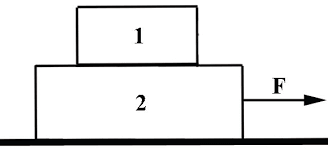
\includegraphics[width=\linewidth]{Problem_31_Figure.png}
\end{minipage}

\category{Dynamics \& Friction}
\StudyGuideLinks{36}
\ProblemSource{36} 
\begin{answerbox}
\finalanswer{(A) $F/(4mg)$}
\end{answerbox}
\begin{insightbox}
Overall acceleration $a=F/(4m)$; the top box requires static friction $F/4$. Compare with $\mu_s mg$ to get the minimum $\mu_s$.
\end{insightbox}
\begin{solutionbox}

Treating both boxes as one: $a=F/(4m)$. For the top box, required static friction $f_s=m a=F/4$. The maximum static friction is $\mu_s mg$, so $F/4\le \mu_s mg \Rightarrow \mu_s=F/(4mg)$.
\end{solutionbox}

% Problem 37
\Needspace{18\baselineskip}
\item \label{prob:37}
A uniform wooden block is a rectangular prism with dimensions of 10 cm x 6 cm x 2 cm. The block will be placed on a level table in one of three possible orientations with a side parallel to the tabletop. Let $P_L$ equal the largest possible pressure the block can exert on the table and $P_S$ equal the smallest possible pressure the block can exert on the table. What is the ratio $P_L/P_S$? 
\begin{enumerate}[label=(\Alph*)]
    \item 5/3
    \item 3
    \item 5
    \item 9
    \item 25
\end{enumerate}

\category{Statics}
\StudyGuideLinks{37}
\ProblemSource{37} 
\begin{answerbox}
\finalanswer{(C) 5}
\end{answerbox}
\begin{insightbox}
Pressure is inversely proportional to contact area; among the three faces the area ratio max/min is $60/12$.
\end{insightbox}
\begin{solutionbox}

Pressure $P=F/A$ with constant weight. Areas: 60, 20, 12 cm$^2$. Ratio $P_L/P_S=A_{max}/A_{min}=60/12=5$.
\end{solutionbox}

% Problem 38
\Needspace{18\baselineskip}
\item \label{prob:38}
A motorcycle has a total mass of 150 kg. Each wheel has a mass of 10 kg and a radius of 30 cm. As the motorcycle is moving, what is the ratio of the rotational kinetic energy of the wheels to the total translational kinetic energy of the motorcycle? Assume the wheels are uniform disks and roll without slipping.
\begin{enumerate}[label=(\Alph*)]
    \item 0.033:1
    \item 0.067:1
    \item 0.33:1
    \item 0.67:1
    \item 3.3:1
\end{enumerate}

\category{Rotational Energy}
\StudyGuideLinks{38}
\ProblemSource{38}
\begin{answerbox}
\finalanswer{(B) $0.067:1$}
\end{answerbox}
\begin{insightbox}
Compare the two wheels' combined rotational energy with the translation of the entire motorcycle.
\end{insightbox}
\begin{solutionbox}
Each wheel (uniform disk) has $I=\tfrac{1}{2}m_w R^2$ and rolls without slipping, so $\omega=v/R$. Thus one wheel's rotational energy is
\[
K_{\text{rot, one}}=\tfrac{1}{2}I\omega^2=\tfrac{1}{2}\Big(\tfrac{1}{2}m_w R^2\Big)\Big(\tfrac{v}{R}\Big)^2=\tfrac{1}{4}m_w v^2.
\]
With two wheels, $K_{\text{rot, wheels}}=2\cdot\tfrac{1}{4}m_w v^2=\tfrac{1}{2}m_w v^2$.

The total translational kinetic energy of the motorcycle (all mass moving at speed $v$) is
\[
K_{\text{trans, total}}=\tfrac{1}{2}M_{\text{total}}v^2.
\]
Therefore the requested ratio is
\[
\frac{K_{\text{rot, wheels}}}{K_{\text{trans, total}}}=\frac{\tfrac{1}{2}m_w v^2}{\tfrac{1}{2}M_{\text{total}}v^2}=\frac{m_w}{M_{\text{total}}}=\frac{10}{150}\approx0.067:1.
\]
\end{solutionbox}

% Problem 39
\Needspace{18\baselineskip}
\item \label{prob:39}
A projectile is launched at an angle of $40^\circ$ above the horizontal with a speed of 30 m/s. Use $g=10\,\mathrm{m/s^2}$. How much time passes before the position of the projectile makes an angle of $20^\circ$ above the horizontal from the original launch point?
\begin{enumerate}[label=(\Alph*)]
    \item 3.02 s
    \item 2.38 s
    \item 2.18 s
    \item 1.93 s
    \item 1.64 s
\end{enumerate}

\category{Kinematics}
\StudyGuideLinks{39}
\ProblemSource{39}
\begin{answerbox}
\finalanswer{(C) $2.18\,\mathrm{s}$}
\end{answerbox}
\begin{insightbox}
The angle of the position vector is found from $y/x$, not from the direction of velocity.
\end{insightbox}
\begin{solutionbox}
Using $x=v_0\cos\theta_0\,t$ and $y=v_0\sin\theta_0\,t-\tfrac12gt^2$, the slope from the origin is
\[
\tan\theta_f=\frac{y}{x}=\tan\theta_0-\frac{g t}{2 v_0\cos\theta_0}.
\]
Solving for $t$ gives
\[
t=\frac{2 v_0 \cos\theta_0}{g}\,(\tan\theta_0-\tan\theta_f)=\frac{2\cdot30\cos40^\circ}{10}\,(\tan40^\circ-\tan20^\circ)\approx2.18\,\text{s}.
\]
\end{solutionbox}
